\documentclass[
size=17pt,
paper=smartboard,
mode=present,
display=slidesnotes,
style=paintings,
nopagebreaks,
blackslide,
fleqn]{powerdot}

% styles: sailor, paintings
% wj capsules prettybox
% mode = handout or present


\usepackage{amsmath,graphicx,color,amsfonts}
\usepackage[brazilian]{babel}
\usepackage[utf8]{inputenc}
\newcommand{\palette}{Europa}


% palettes:
%    - sailor: Sea, River, Wine, Chocolate, Cocktail 
%    - paintings: Syndics, Skater, GoldenGate, Moitessier, PearlEarring, Lamentation, HolyWood, Europa, MayThird, Charon 

\newcommand{\cursopequeno}{EC01008 AOC}
\newcommand{\cursogrande}{\Large EC01008 -- Arquitetura e organização de computadores}



\author{Ronaldo de Freitas Zampolo\\FCT-ITEC-UFPA}
\date{2023-4}


\pdsetup{
   lf = {\cursopequeno},
   rf = {Memória interna}, palette = {\palette}, randomdots={false},
   cf = {\theslide}
}


%opening
\title{\cursogrande\\ \vspace{1cm}{Memória interna}}

\begin{document}
\maketitle[randomdots={false}]

\begin{slide}{Agenda}
      \tableofcontents[content=sections]
   \end{slide}

\section[slide=true]{Memória principal semicondutora}
\begin{slide}{Organização}
   \begin{itemize}
      \item Elemento básico: célula de memória
      \item Propriedades das células de memória:
      \begin{itemize}
         \item Dois estados: 0 e 1
         \item Passíveis de serem escritas (pelo menos uma vez) para definir o estado
         \item Podem ser lidas para verificação do estado
      \end{itemize}
      \begin{figure}[h]
         \centering
         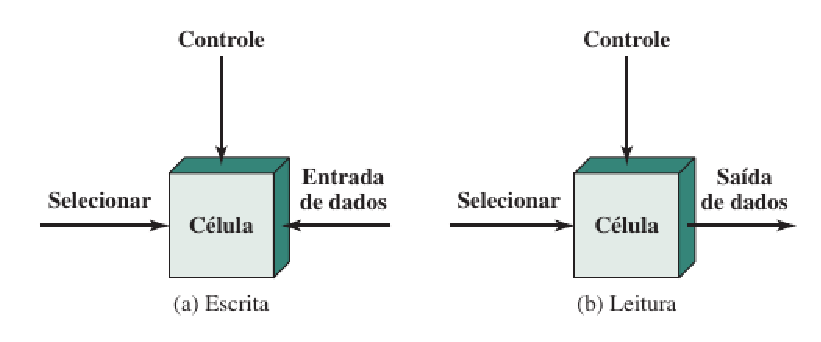
\includegraphics[width=0.7\textwidth]{figs/celula2}
      \end{figure}
   \end{itemize}
\end{slide}

\begin{slide}{DRAM e SRAM}
   \begin{itemize}
      \item Memória de acesso aleatório: palavras individuais são acessadas diretamente por meio da lógica de endereçamento interna
      \item Tipos de memória semicondutora:
      \begin{figure}[h]
         \centering
         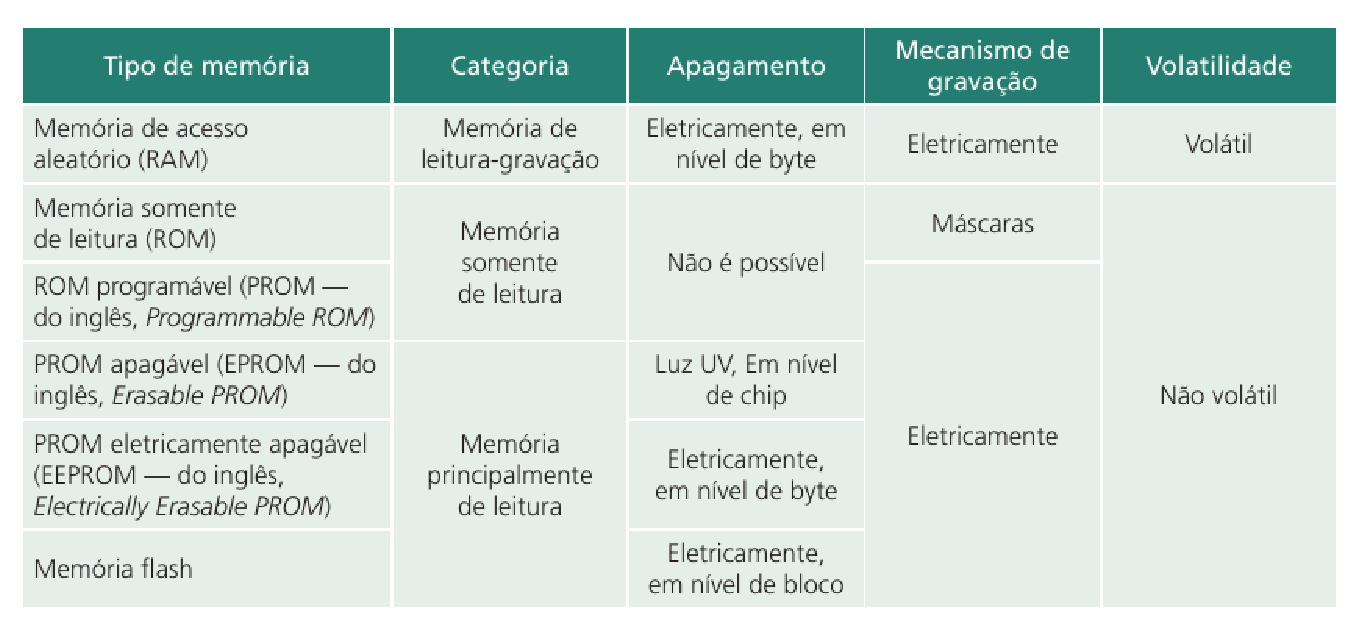
\includegraphics[width=0.9\textwidth]{figs/tipos2}
      \end{figure}
   \end{itemize}
\end{slide}

\begin{slide}{DRAM e SRAM}
   \begin{itemize}
      \item RAM dinâmica (DRAM):
      \begin{itemize}
         \item Células de memória utilizam capacitores
         \item Dados são armazenados como cargas em capacitores
         \item Problema: perda de carga do capacitor
         \item Solução: circuitos para recarga periódica
      \end{itemize}
      \item RAM estática (SRAM):
      \begin{itemize}
         \item Células de memória baseadas em \textit{flip-flop}
         \item Não há necessidade de recarga periódica
      \end{itemize}
   \end{itemize}
\end{slide}

\begin{slide}{DRAM e SRAM}
   \begin{itemize}
      \item SRAMs e DRAMs são ambas voláteis;
      \item As células de memória das DRAMs são menores e mais simples;\pause
      \item Logo, as DRAMs são mais densas e mais baratas que SRAMs correspondentes;\pause
      \item SRAMs são mais rápidas que DRAMs; \pause
      \item Em geral, DRAMs são usadas na memória principal e as SRAMs na memória cache
   \end{itemize}
\end{slide}

\begin{slide}{Tipos de ROM}
\begin{itemize}
   \item ROM
   \begin{itemize}
      \item Contém um padrão de bits que não pode ser mudado (não volátil, gravação física);
      \item Aplicações: microprogramação, biblioteca de uso frequente, programas do sistema, tabelas de função
      \item Custo alto e relativamente fixo, independente do número de unidades fabricadas
      \item Sem espaço para erro
   \end{itemize}
   \item PROM 
   \begin{itemize}
      \item Pode ser escrita apenas uma vez (equipamento especial);
      \item Mais flexível e atraente para grandes volumes
   \end{itemize}

\end{itemize}

\end{slide}

\begin{slide}{Tipos de ROM}
\begin{itemize}
   \item EPROM
   \begin{itemize}
      \item Leitura e escrita por processos elétricos;
      \item Pode ser escrita mais de uma vez (precisa ser apagada primeiro);
      \item Para apagar: exposição à luz ultravioleta (15 a 20 minutos)
      \item Mais cara que a PROM
   \end{itemize}
   \item EEPROM 
   \begin{itemize}
      \item Leitura e escrita por processos elétricos;
      \item Somente os bytes endereçados são atualizados;
      \item Mais cara e menos densa que as EPROMs
   \end{itemize}
\end{itemize}
\end{slide}

\begin{slide}{Tipos de ROM}
\begin{itemize}
   \item Memória \textit{flash}
   \begin{itemize}
      \item Tecnologia elétrica de apagamento (como a EEPROM)
      \item Velocidade de apagamento muito superior
      \item Apagamento de blocos e não da memória inteira
      \item Não oferece apagamento em nível de byte
   \end{itemize}
\end{itemize}
\end{slide}

\begin{slide}{Lógica do chip}
\begin{itemize}
   \item Escolhas quanto à organização das células de memória e  à lógica funcional \pause
   \item Uma DRAM de 16 Mbits: \pause
   \begin{itemize}
      \item Memória de 1 M endereços de 16 bits cada\pause
      \item Memória de 16 M endereços de 1 bit cada\pause
      \item Configurações intermediárias (Ex.: 2 K $\times$ 2 K $\times$ 4 bits)
   \end{itemize}
\end{itemize}
\end{slide}

\begin{slide}{Lógica do chip}
\begin{figure}[h]
         \centering
         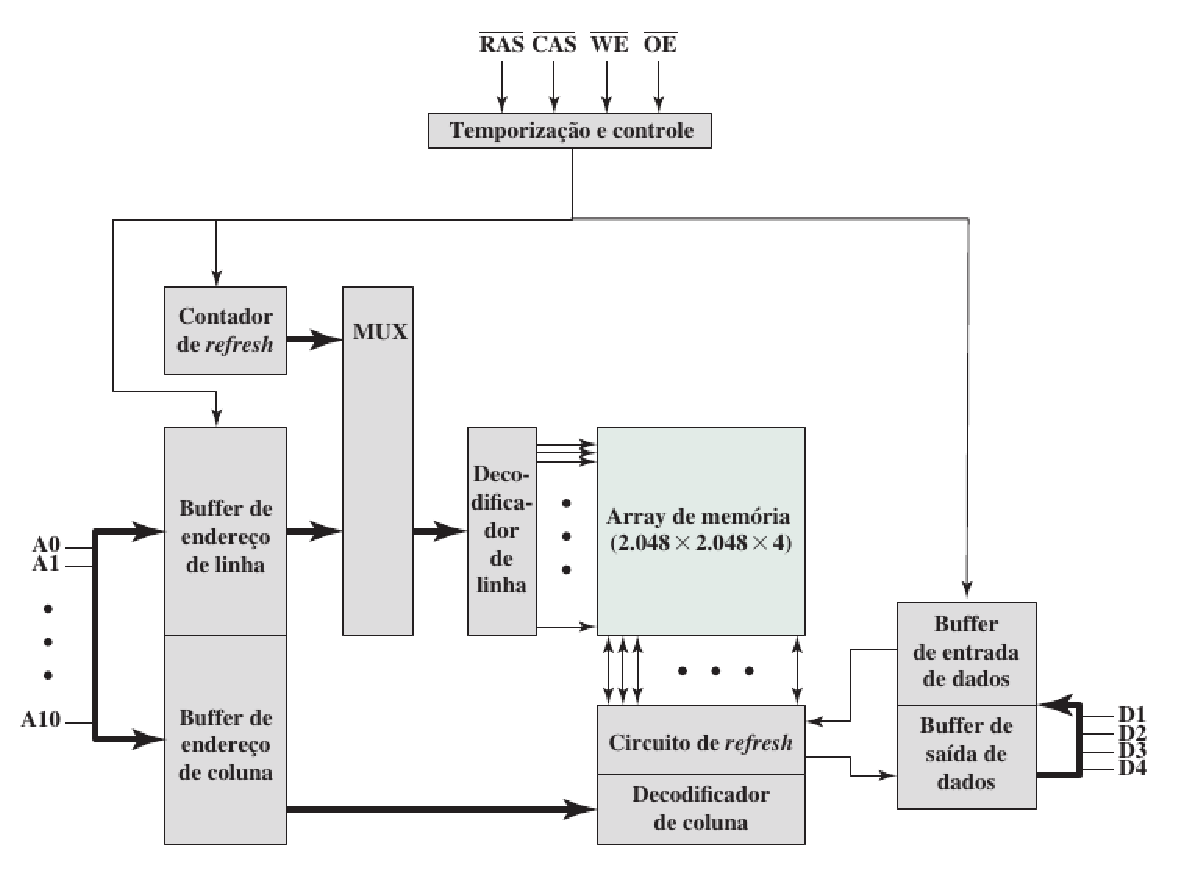
\includegraphics[width=0.70\textwidth]{figs/dram_tip2}
      \end{figure}
\end{slide}

\begin{slide}{Empacotamento do chip}
\begin{figure}[h]
         \centering
         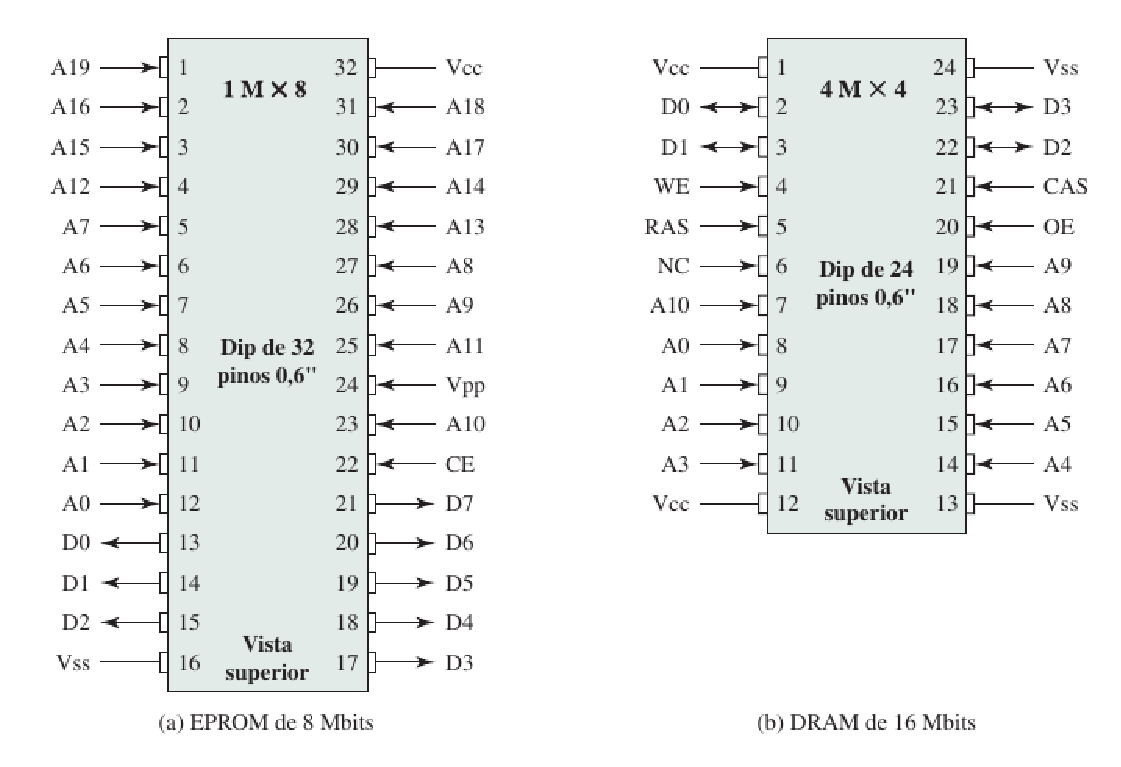
\includegraphics[width=0.70\textwidth]{figs/empacotamento2}
      \end{figure}
\end{slide}

\begin{slide}{Organização do módulo}
\begin{figure}[h]
         \centering
         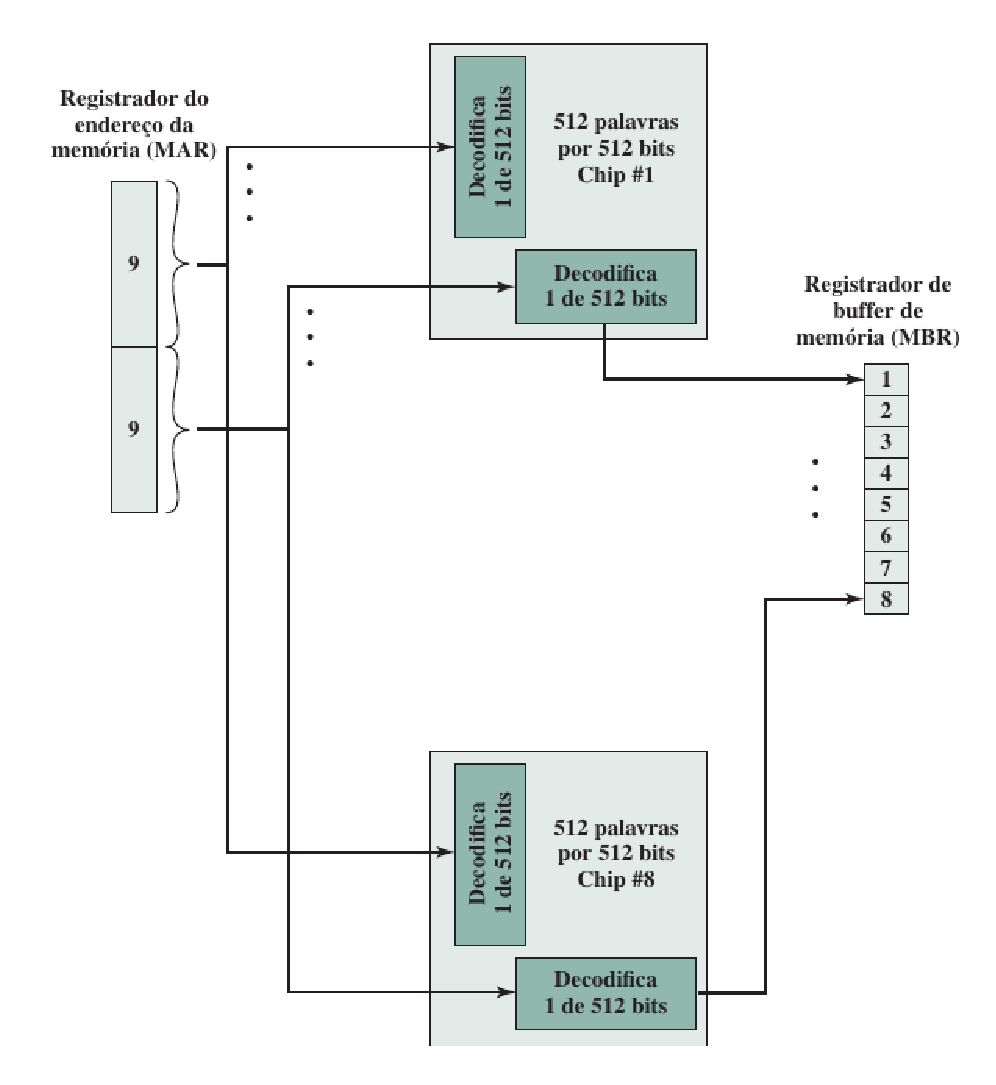
\includegraphics[height=0.8\textheight]{figs/org_m256k2}
      \end{figure}
\end{slide}

\begin{slide}{Organização do módulo}
\begin{figure}[h]
         \centering
         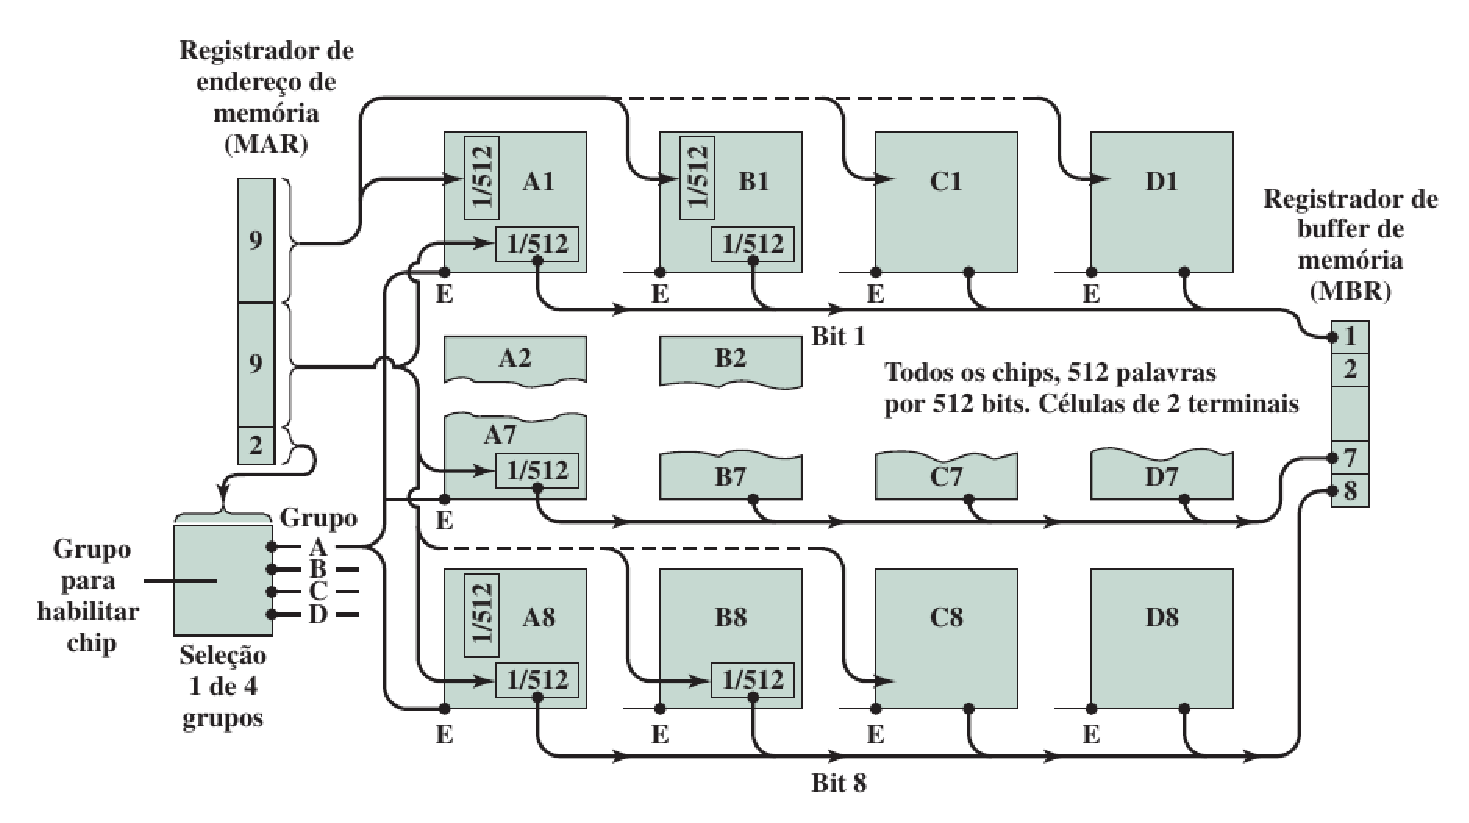
\includegraphics[width=0.9\textwidth]{figs/org_m1M2}
      \end{figure}
\end{slide}

\section[slide=true]{Correção de erro}

\begin{slide}{Erros em sistemas de memória}
\begin{itemize}
   \item Um sistema de memória semicondutora está sujeito a erros\pause
   \item Tipos de erros: \pause
   \begin{itemize}
      \item Falha permanente: defeito físico, causado por uso intenso em ambiente impróprio, defeitos de fabricação ou desgaste \pause
      \item Erro não permanente: eventos aleatórios que alteram os bits armazenados sem danificar as memórias, tais como defeitos na fonte de alimentação, interferências, etc.
   \end{itemize}
\end{itemize}
\end{slide}

\begin{slide}{Processo de correção de erro}
\begin{figure}[h]
         \centering
         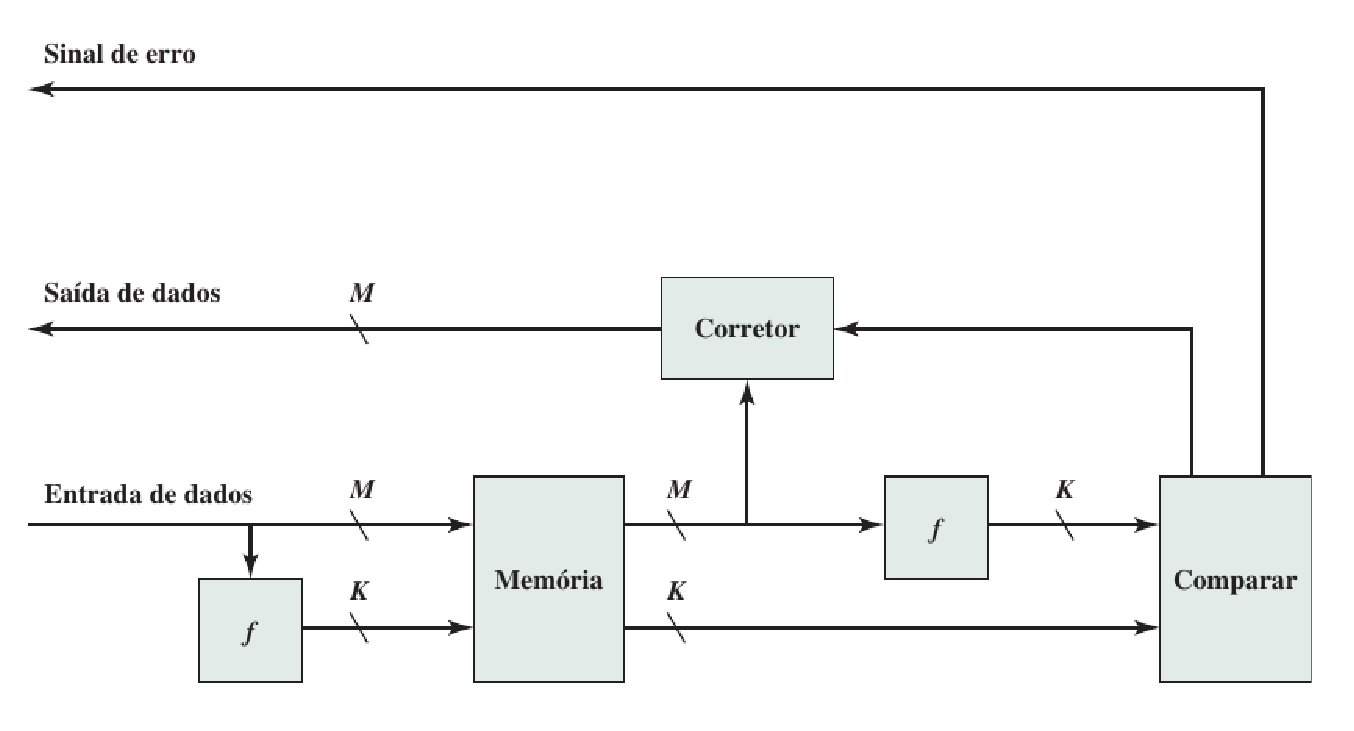
\includegraphics[width=0.9\textwidth]{figs/correrro2}
      \end{figure}
\end{slide}

\begin{slide}{Processo de correção de erro}
\begin{itemize}
   \item Comprimento da mensagem (M): m bits
   \item Comprimento do código (K): k bits
   \item Tamanho total armazenado: m+k bits\pause
   \item Três situações:\pause
   \begin{itemize}
      \item Nenhum erro é detectado\pause
      \item Um erro é detectado e é possível corrigi-lo\pause
      \item Um erro é detectado, mas não é possível corrigi-lo
   \end{itemize}
\end{itemize}
\end{slide}

\begin{slide}{Código de Hamming}
\begin{itemize}
   \item Idealizado por Richard Hamming (Bell Labs, 1950)
   \item O mais simples dos códigos de correção
   \item Exemplo para $m=4$, usando diagramas de Venn (1881, por John Venn, matemático britânico, 1834-1923)\\
   \begin{figure}[h]
      \centering
      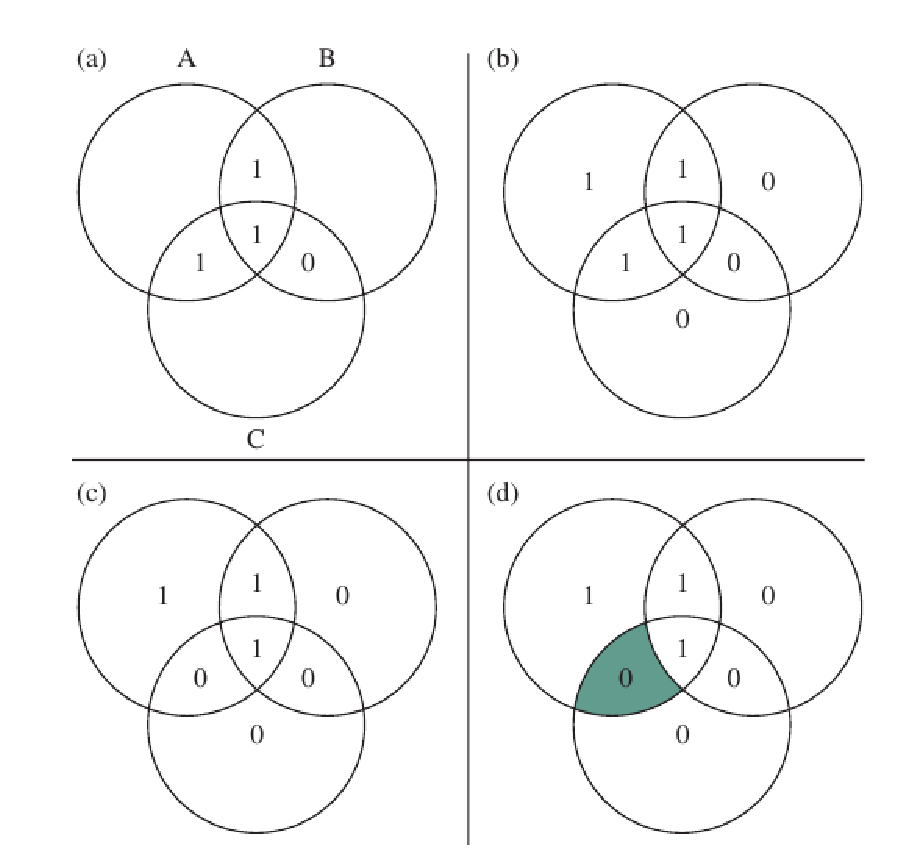
\includegraphics[height=0.5\textheight]{figs/venn1-2}
   \end{figure}
\end{itemize}
\end{slide}

\begin{slide}{Código de Hamming}
\begin{itemize}
   \item Exemplo: código para detectar e corrigir erros em palavras de 8 bits ($m=8$)\pause
   \item Bloco de comparação: operação lógica XOR
   \begin{equation*}
       s = k_1 \text{ XOR } k_2,
   \end{equation*}
   onde $s$ é denominado \emph{palavra síndrome}\pause
   \item $s = 0$: nenhum erro foi detectado\pause
   \item $s \neq 0$: erro(s) foi(foram) detectado(s)\pause
   \item $2^k -1$ valores de $s$ para indicar erro e sua localização:
   \begin{equation*}
      2^k -1 \geq m+k
   \end{equation*}
\end{itemize}
\end{slide}

\begin{slide}{Código de Hamming}
\begin{itemize}
   \item 8 bits de dados exigem 4 bits de verificação
   \begin{figure}[h]
      \centering
      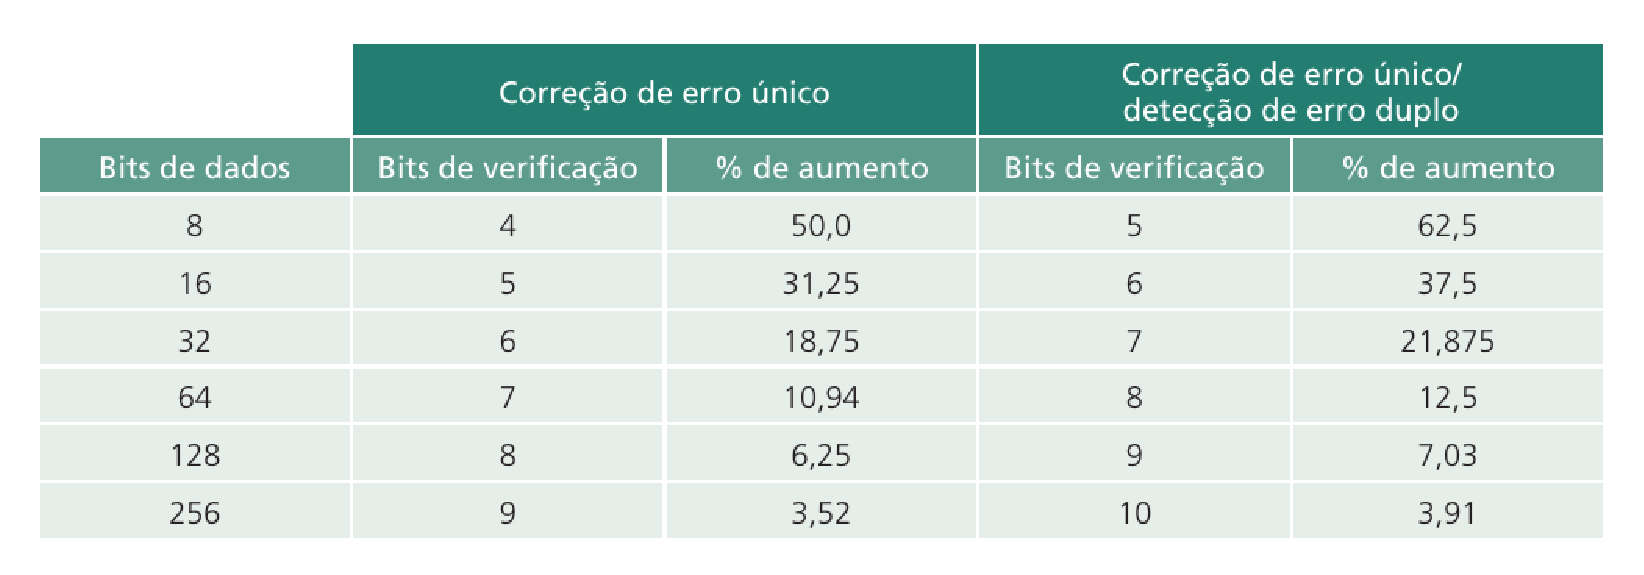
\includegraphics[width=0.9\textwidth]{figs/tabhamm2}
   \end{figure}
\end{itemize}
\end{slide}

\begin{slide}{Código de Hamming}
\begin{itemize}
   \item Características desejadas:\pause
   \begin{itemize}
      \item $s$ contém somente zeros: nenhum erro detectado\pause
      \item $s$ contém apenas um bit 1: erro no código, não há necessidade de correção\pause
      \item $s$ contém mais de um bit 1: erro na mensagem, valor numérico de $s$ indica a posição
   \end{itemize}
\end{itemize}
\begin{figure}[h]
         \centering
         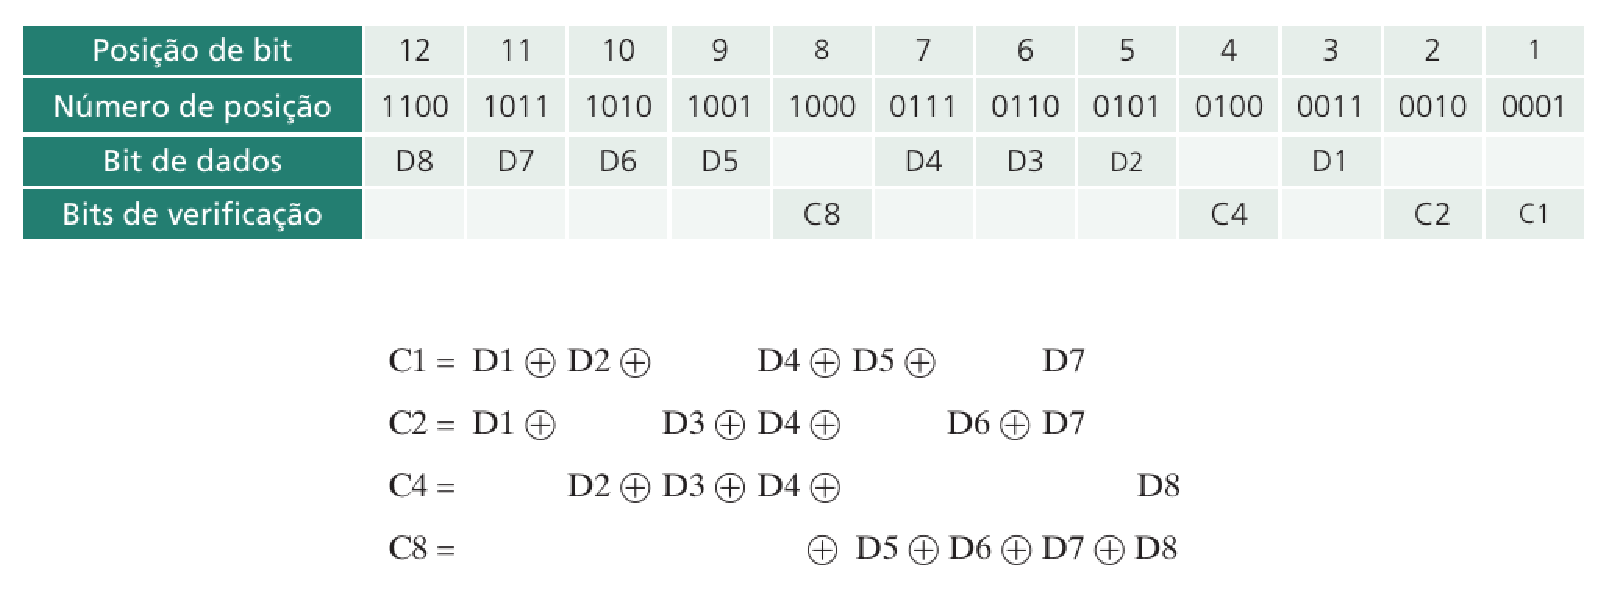
\includegraphics[width=0.9\textwidth]{figs/layout2}
      \end{figure}
\end{slide}

\begin{slide}{Código de Hamming}
\begin{itemize}
   \item Determinação da palavra código:
   \begin{tabular}{l l l l l l l l l}
      C1 = &D1$\oplus$ &D2$\oplus$ &           &D4$\oplus$ &D5$\oplus$ &           &D7 &    \\
      C2 = &D1$\oplus$ &           &D3$\oplus$ &D4$\oplus$ &           &D6$\oplus$ &D7 &    \\
      C4 = &           &D2$\oplus$ &D3$\oplus$ &D4$\oplus$ &           &           & & D8 \\
      C8 = &           &           &           &           &D5$\oplus$ &D6$\oplus$ &D7$\oplus$ & D8 \\
   \end{tabular}
   \item Exemplo: 
   \begin{itemize}
      \item mensagem (D8 D7 D6 D5 D4 D3 D2 D1)= 00111001
      \item palavra código (C8 C4 C2 C1) = 0111
      \item mensagem + código = 0011\textcolor{red}{0}100\textcolor{red}{1}1\textcolor{red}{1}\textcolor{red}{1}
   \end{itemize}
\end{itemize}
\end{slide}

\begin{slide}{Código de Hamming}
\begin{itemize}
   \item Exemplo (continuação): 
   \begin{itemize}
      \item mensagem (D8 D7 D6 D5 D4 D3 D2 D1)= 00111001
      \item palavra código (C8 C4 C2 C1) = 0111
      \item mensagem + código = 0011\textcolor{red}{0}100\textcolor{red}{1}1\textcolor{red}{1}\textcolor{red}{1}\pause
      \item 1º caso: inversão do bit C4; \pause 
      \item 2º caso: inversão do bit D4;\pause
      \item 3º caso: inversão dos bits D3 e D4;\pause 
      \item 4º caso: inversão dos bits C4, D3 e D4 \pause
      \item 5º caso: inversão dos bits D1, D3 e D4
   \end{itemize}
\end{itemize}
\end{slide}

\begin{slide}{Código de Hamming}
\begin{itemize}
   \item Abordagem SEC-DED: 
   \begin{itemize}
      \item Estratégia usualmente implementada em memórias semicondutoras;
      \item Exige 1 bit a mais em relação à SEC
   \end{itemize}
   \begin{figure}[h]
      \centering
      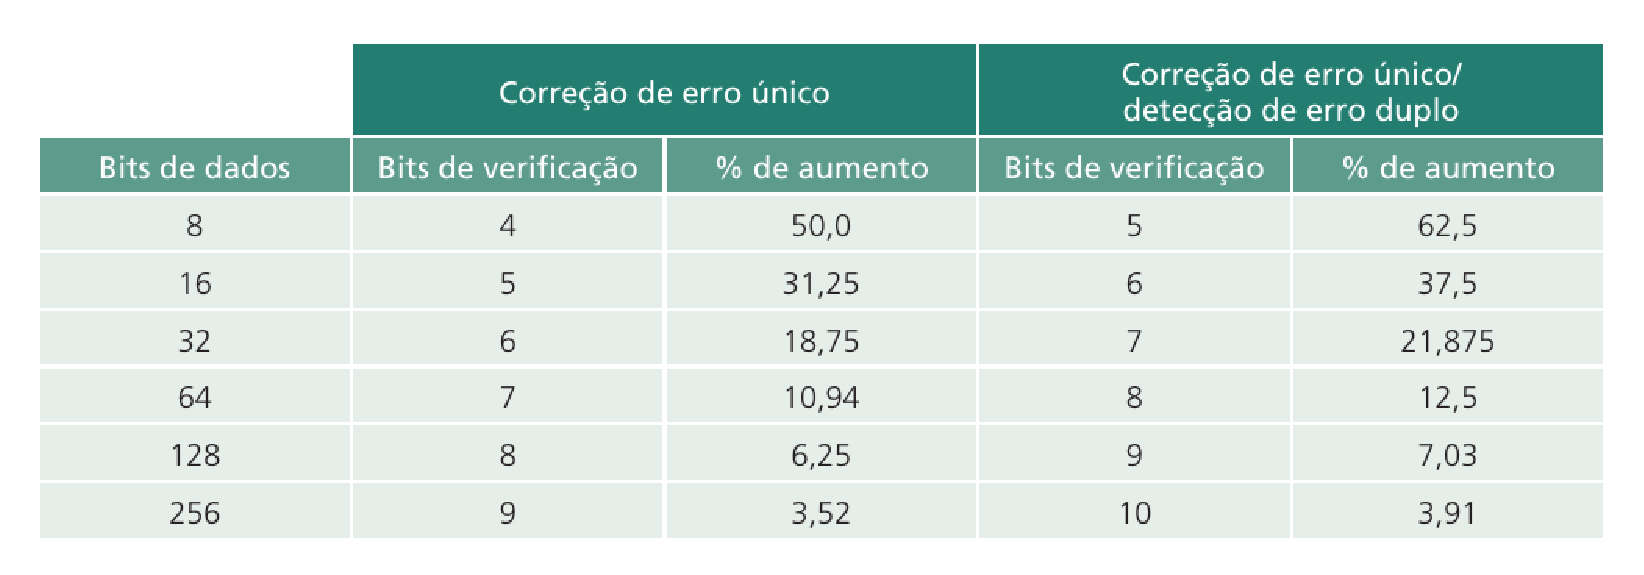
\includegraphics[width=0.9\textwidth]{figs/tabhamm2}
   \end{figure}
\end{itemize}
\end{slide}

\begin{slide}{Código de Hamming}
\begin{itemize}
   \item Abordagem SEC-DED (continuação): 
   \begin{figure}[h]
      \centering
      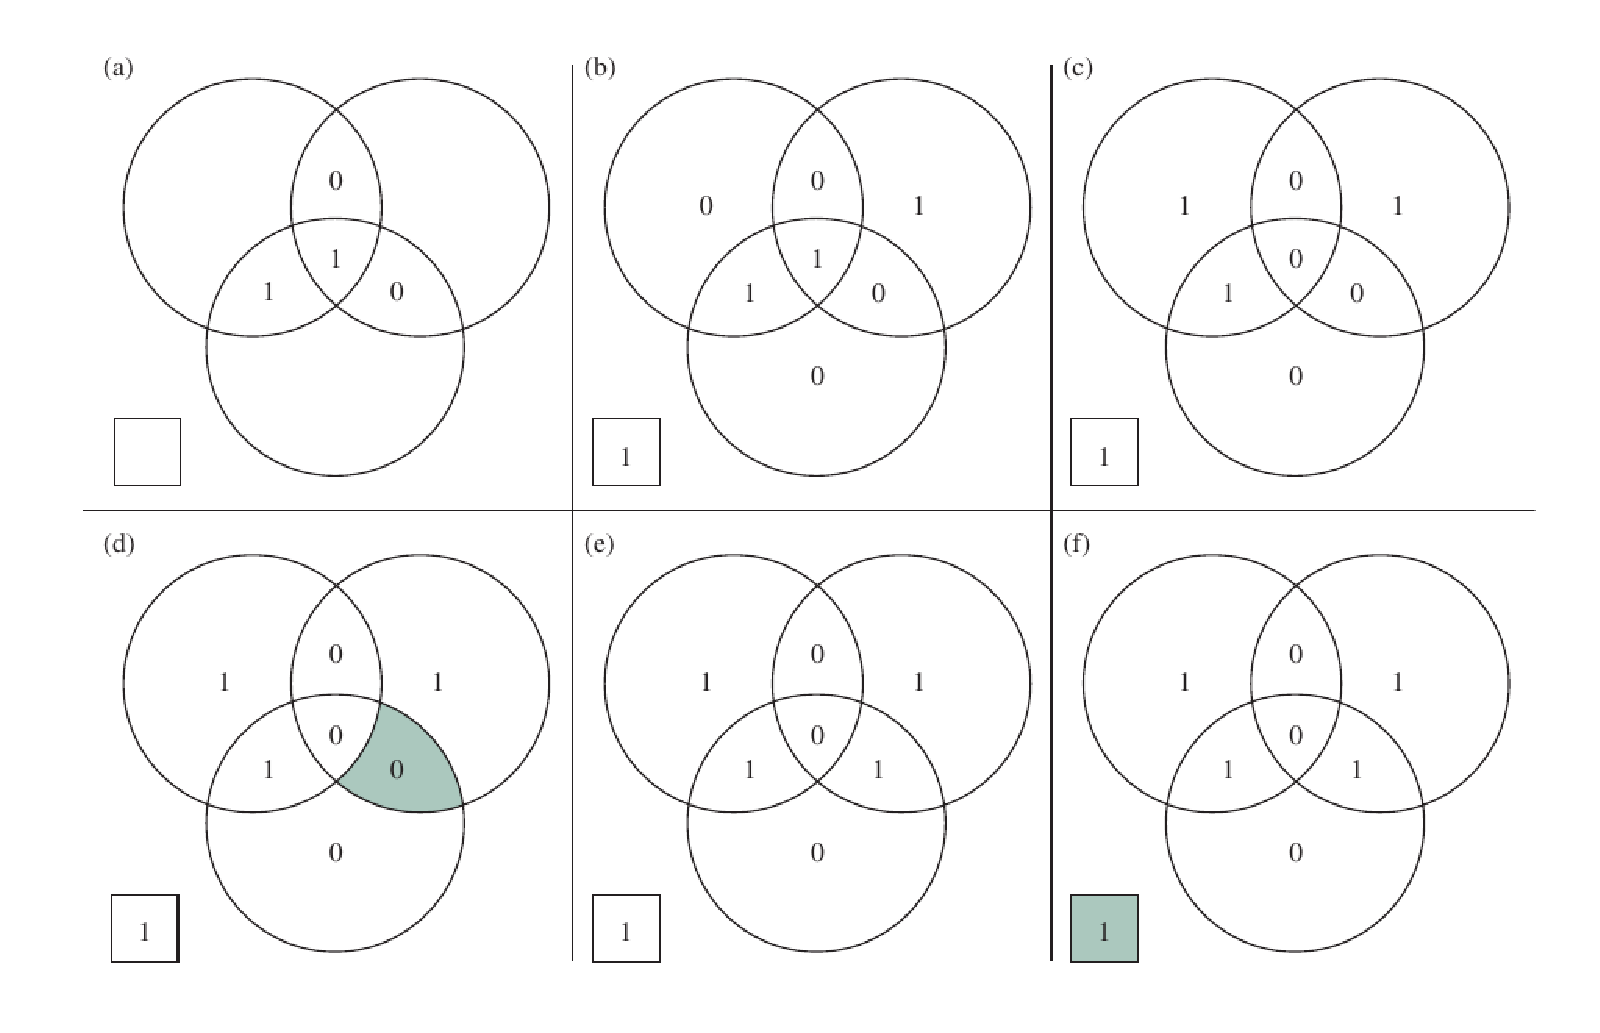
\includegraphics[width=0.75\textwidth]{figs/venn3}
   \end{figure}
\end{itemize}
\end{slide}

\section[slide=true]{Organizações avançadas de DRAM}
\begin{slide}{Ainda custo $\times$ desempenho}
   \begin{itemize}
      \item Interface processador-memória principal: caminho mais importante do sistema
      \item Inserção de cache: 
	      \begin{itemize}
		      \item SRAM muito mais cara que a DRAM
		      \item A partir de um certo ponto não compensa (\emph{diminishing returns})
	      \end{itemize}
      \item Mudanças na arquitetura básica da DRAM 
	      \begin{itemize}
		      \item DRAM síncrona (SDRAM)
		      \item DDR SDRAM
	      \end{itemize}
      %\begin{figure}[h]
      %\centering
      %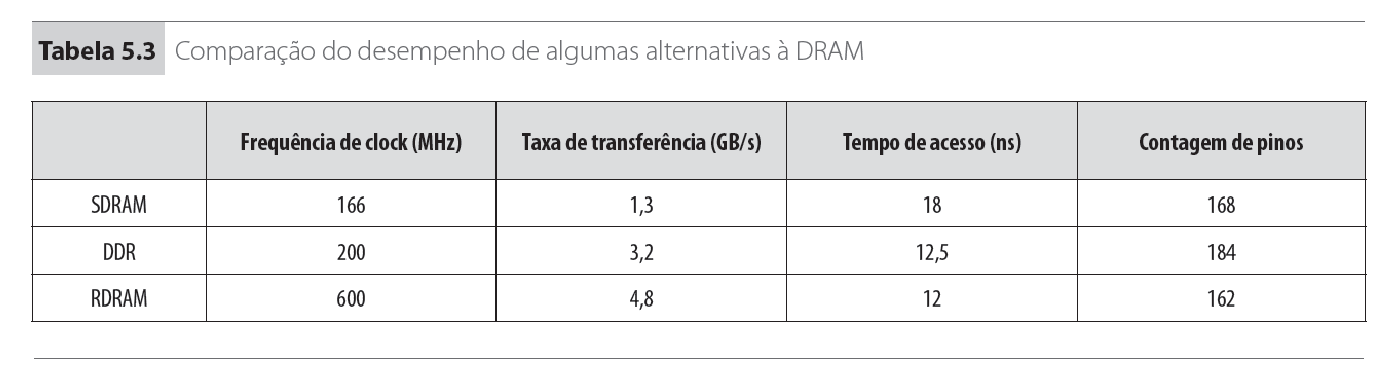
\includegraphics[scale=0.55]{figs/tabdram}
   %\end{figure}
   \end{itemize}
\end{slide}
 
 \begin{slide}{DRAM síncrona (SDRAM)}
 \begin{itemize}
    \item Troca de dados com o processador sincronizada com um clock externo
    \item Modo rajada: elimina o tempo de configuração de endereços
    \item Arquitetura de banco múltiplo
    \begin{figure}[h]
       \centering
%       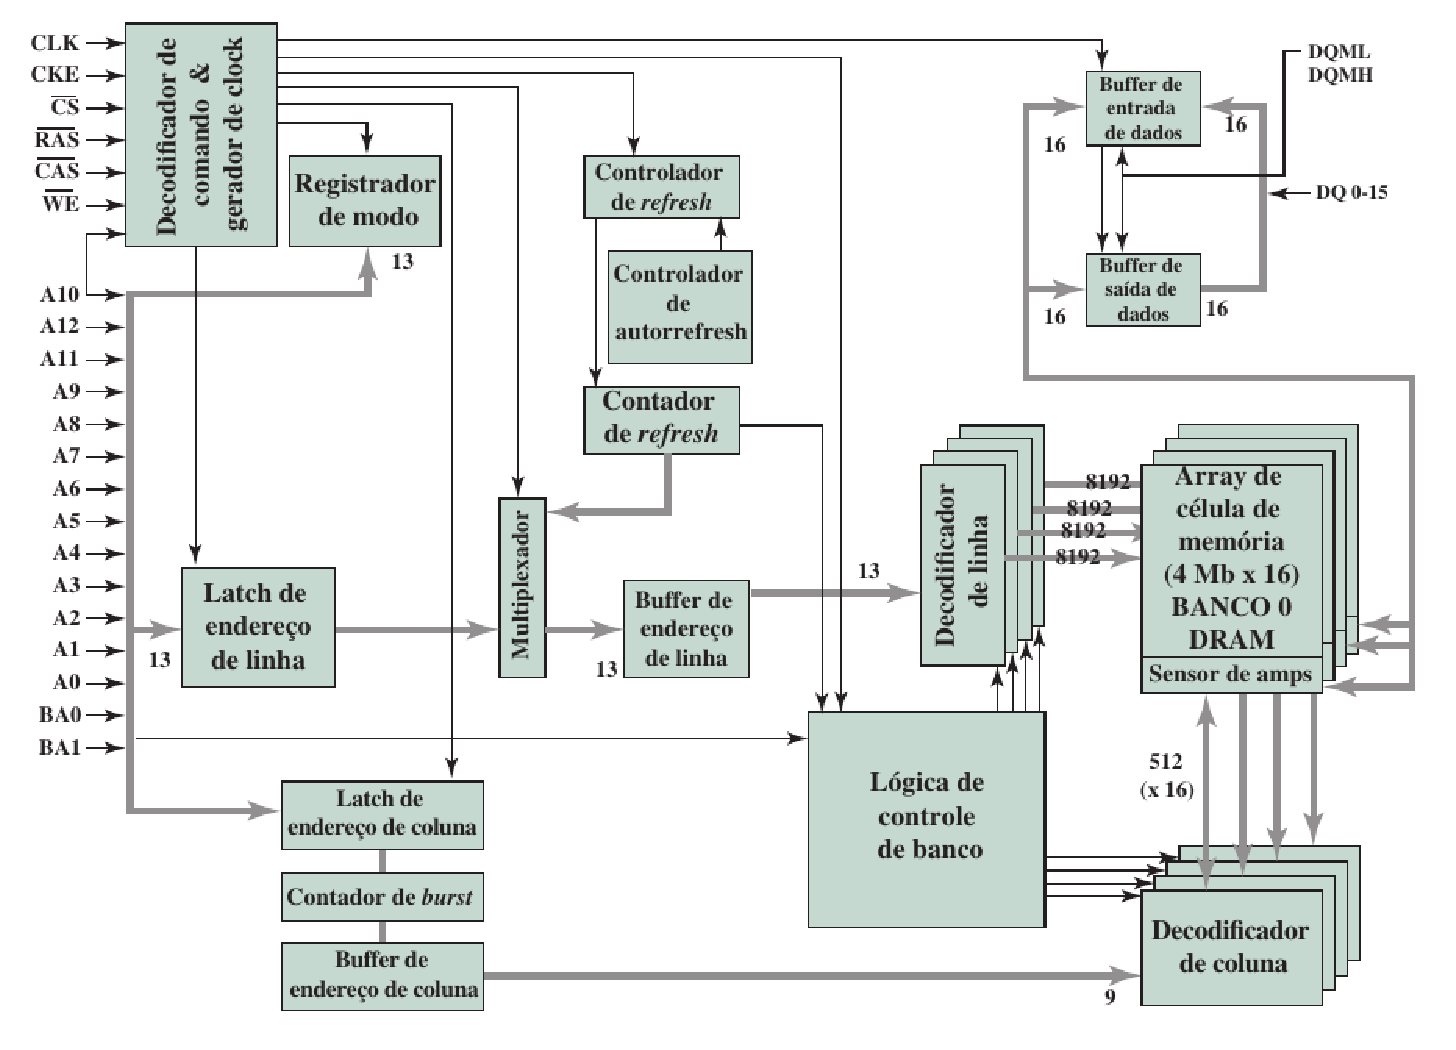
\includegraphics[width=0.55\textwidth]{figs/sdram}
       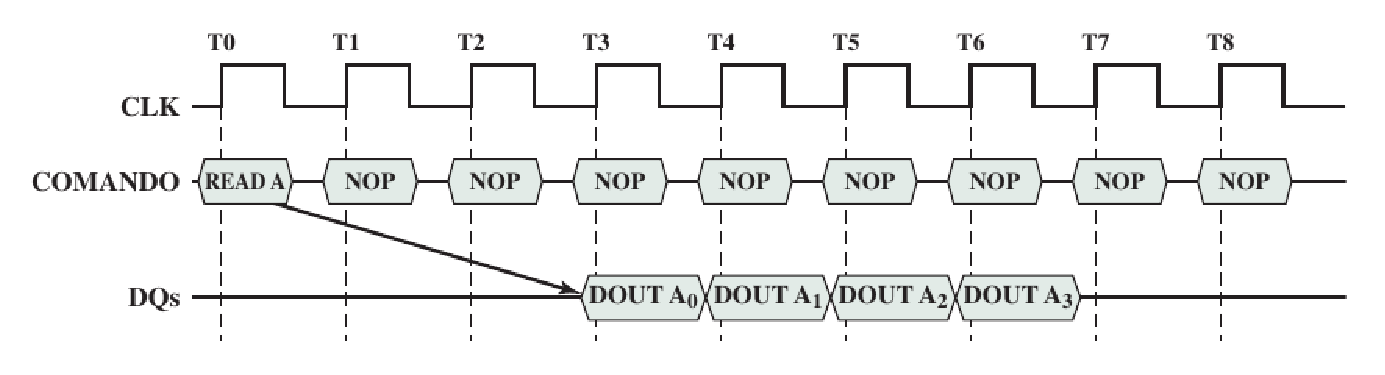
\includegraphics[width=0.85\textwidth]{figs/sdram-temp}
    \end{figure}
 \end{itemize}
 \end{slide}
 
 \begin{slide}{DRAM síncrona (SDRAM)}
 \begin{itemize}
    \item Diagrama de uma SDRAM
    \begin{figure}[h]
       \centering
       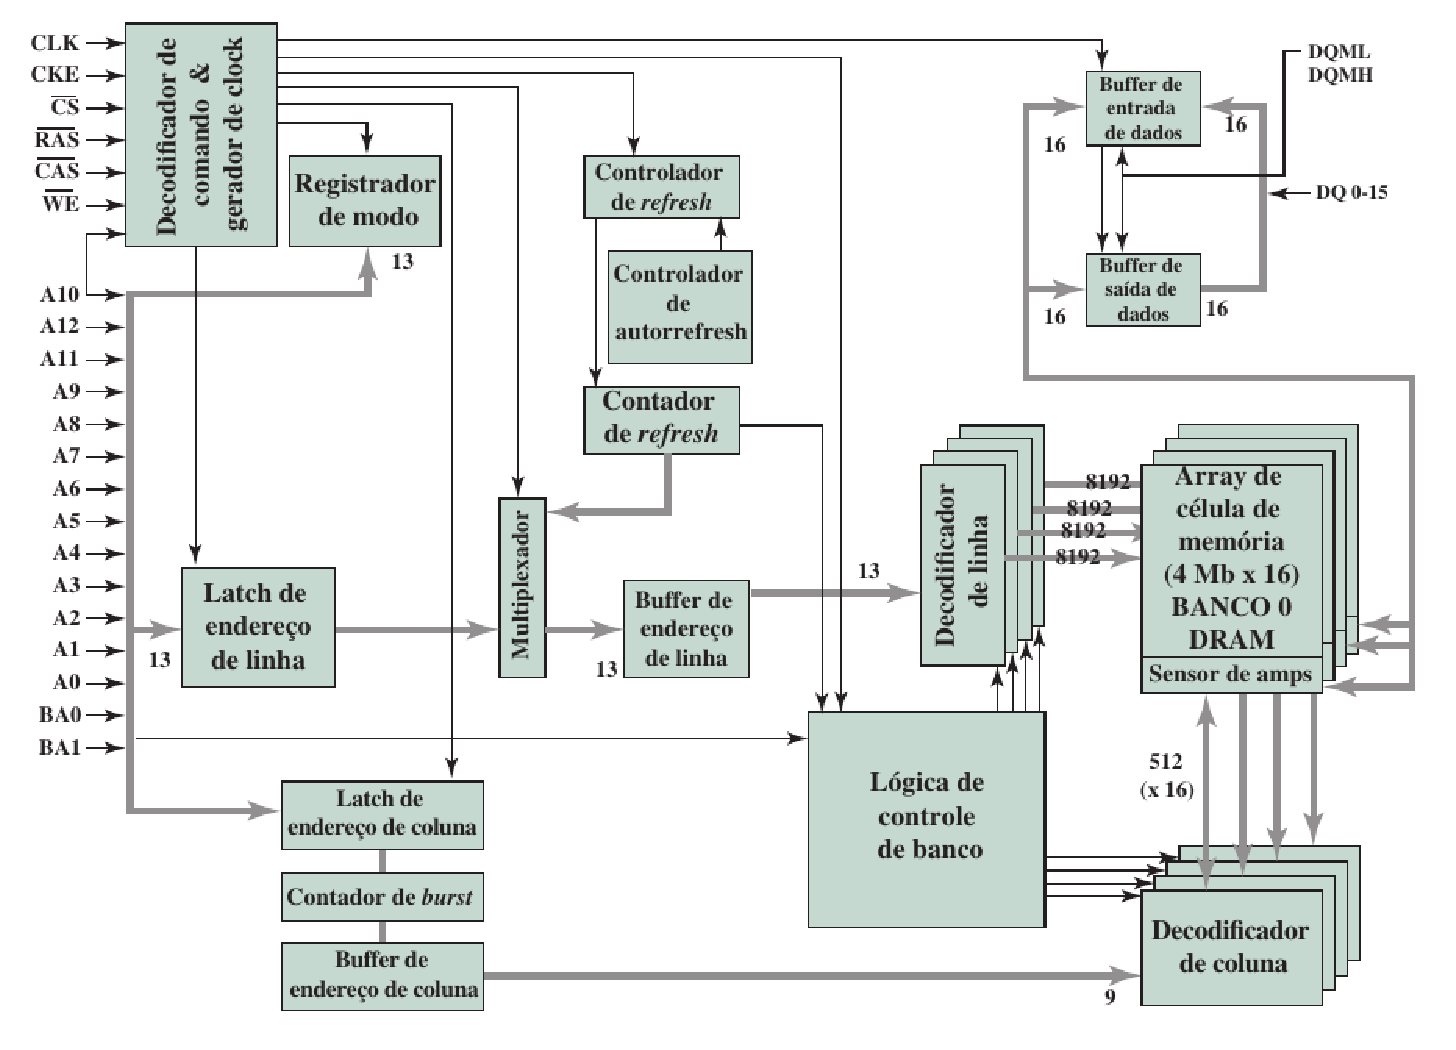
\includegraphics[width=0.65\textwidth]{figs/sdram}
    \end{figure}
 \end{itemize}
 \end{slide}

\begin{slide}{Double Data Rate SDRAM (DDR-SRAM)}
	\begin{itemize}
		\item Fatores que justificam a maior taxa de dados em DDRs:
			\begin{itemize}
				\item Sincronização sensível à subida e descida do sinal de clock
				\item Taxa de clock maior no barramento
				\item Esquema de armazenamento temporário de dados (espécie de cache interna da memória)
			\end{itemize}
	\end{itemize}
	\begin{figure}[h]
		\centering
		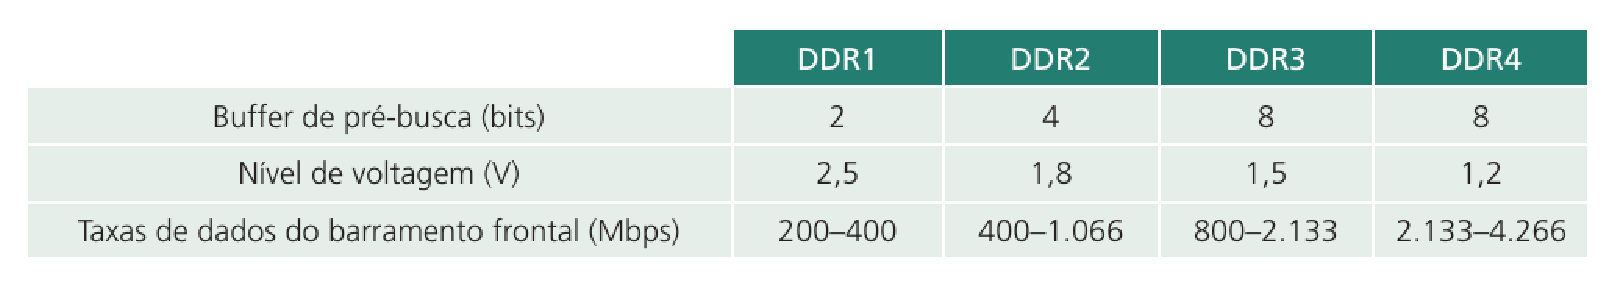
\includegraphics[width=0.9\textwidth]{figs/ddr-caracteristicas}
	\end{figure}

\end{slide}

\begin{slide}{Double Data Rate SDRAM (DDR-SRAM)}
	\begin{itemize}
		\item Gerações de DDR 
	\end{itemize}
	\begin{figure}[h]
		\centering
		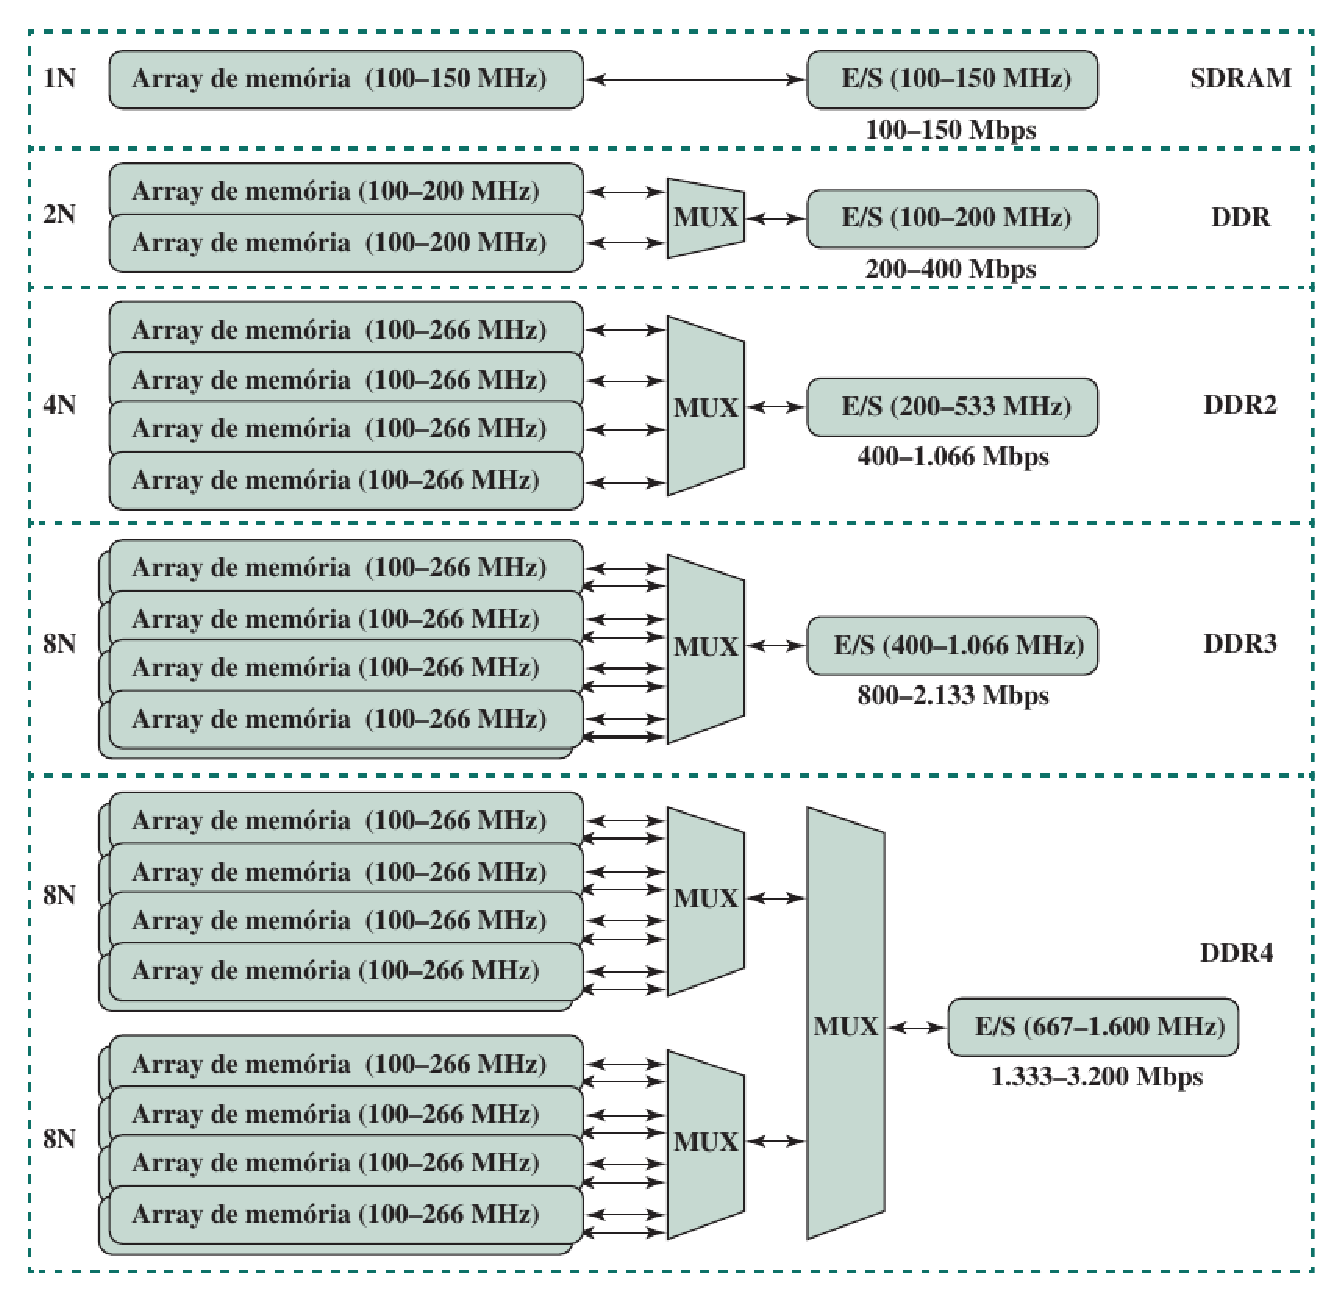
\includegraphics[width=0.5\textwidth]{figs/ddr}
	\end{figure}
\end{slide}

% \section[slide=True]{Memória flash}
% \begin{slide}{Memória flash}
% \end{slide}
%
% \section[slide=True]{Novas tecnologias de memórias de estado sólido não-voláteis}
% \begin{slide}{STT-RAM}
% \end{slide}
%
% \begin{slide}{PCRAM}
% \end{slide}
%
% \begin{slide}{ReRAM}
% \end{slide}
%


\end{document}
